Similar to previous approaches, we simulated two parent signals of size $10^5$ with a set number of structural variants and a set similarity of $80\%$ between the parent signals \cite{MB_diploidTrios, MB_SingleParentDiploid}. In the parent signals, $5000$ locations were chosen at random to be structural variants. We then constructed the child signal by first applying a logical implementation of inheritance to $\lfloor 5000p \rfloor$ randomly selected parent structural variants (where $p$ is the percent overlap between parent and child SVs). Next, we chose  $(5000 - \lfloor 5000p \rfloor)$ locations from the remaining $(10^5 - 5000)$ that were not chosen as a parent variant to be novel variants in the child.  After forming the true signals for each individual, the observed signals were generated by sampling from the Negative Binomial distribution with a given coverage and error.For the purpose of testing the proposed approach, only one parent signal was used. The data simulation code was implemented in Python. \\\\
%Specifically, we used a logical implementation of inheritance (e.g. if both parents were homozygous for a variant, then the child would also be homozygous and so on) with a parent similarity of $80\%$.
\textbf{Analysis.} Given an optimal $\tau, \gamma$ values, our method is better able to reconstruct the homozygous signals for each individual despite large sequencing and mapping error, $\varepsilon = 0.5$. In Figure \ref{fig:results} we show both Receiving Operating Characteristic (ROC) and Precision-Recall (PR) curves obtained for a simulated data set where the parents share $80\%$ of their SVs. Similar to previous work, we use the area under the curve (AUC) for the ROC curves to measure the ability of SPIRAL and NEBULA to distinguish between classes. % say something about NEBULA showing improvements to SPIRAL
Since SVs are very rare and we are faced with strongly imbalanced data, however, we incorporate Precision-Recall curves to gain a deeper understanding of the performance of our algorithm as it relates to false positives \cite{saito2015precision}. We see improvements in area under the curve and average precision for the parent and child's inherited signals. We also see comparable performance for the reconstruction of the child's novel signal.

\begin{figure}[t]
	
	\begin{minipage}[t]{1.0\linewidth}
		\centering
		\centerline{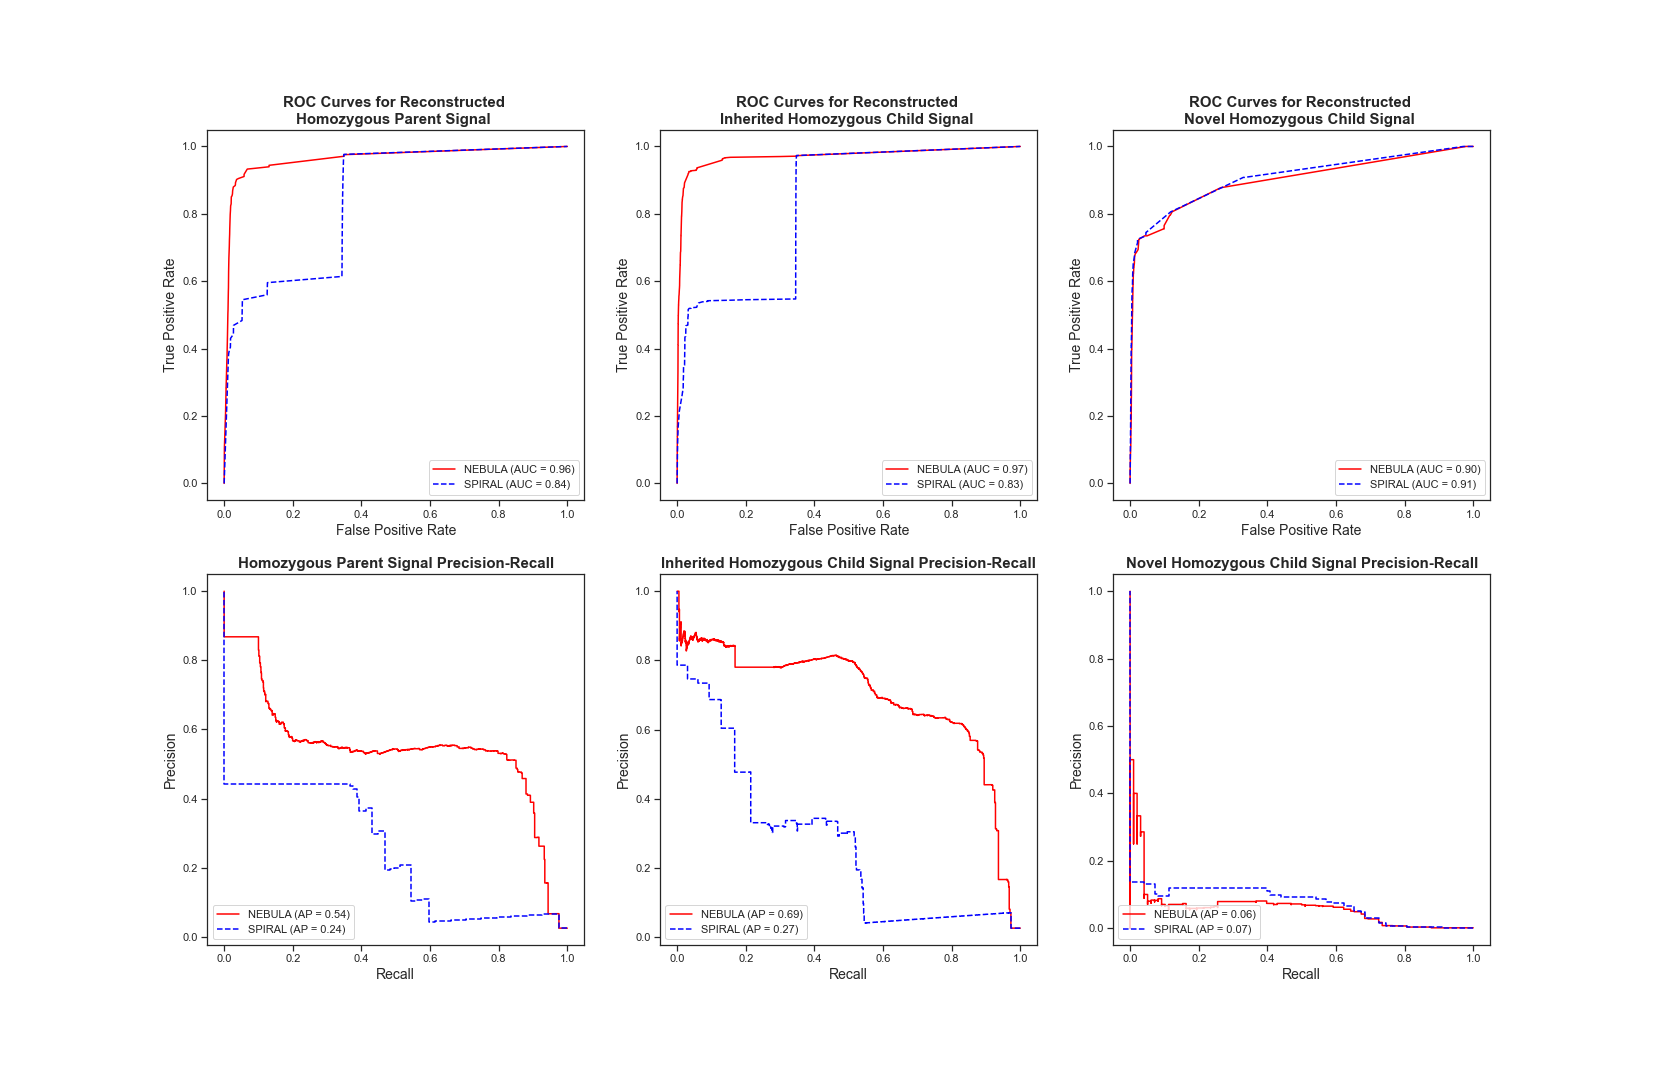
\includegraphics[width=\textwidth]{figs/results_100000n_5000k_7Lp_3Lc_diploid_4pctNovel_80pctSim_5e-01eps_1tau_2gamma_RESULTS}}
		%  \vspace{2.0cm}
	%	\centerline{(a) Result 1}\medskip
	\end{minipage}
	
	\caption{ROC and PR curves of two methods illustrating the area under the curve and average precision in the parent and child reconstruction signals where $\tau = 1, \, \gamma = 2$. The coverage values for each signal are as follows $(\lambda_P, \lambda_P) = (7,3)$ and sequencing error $\varepsilon = 0.5.$}
	\label{fig:results}
	%
\end{figure}